 \documentclass[12pt, a4paper]{article}
\usepackage[utf8]{inputenc}
\usepackage{amsmath, amssymb, amsthm, amsfonts}
\usepackage{CJKutf8}
\usepackage{tikz}
\usetikzlibrary{calc}
\usetikzlibrary{arrows.meta, patterns}
\usepackage[margin=1in]{geometry}
\newtheorem{lemma}{Lemma}
\newcommand{\R}{\mathbb{R}}
 
\newenvironment{solution}
  {\paragraph{\textit{Solution:}}\par\medskip}
  {\hfill$\blacksquare$\vspace{0.1cm}}

\title{Topics in Geometry and Topology:Assignment 5}
\author{
    \begin{CJK*}{UTF8}{gbsn}
    钟皓宇 (12533556)
    \end{CJK*}
}
\date{\today}

\begin{document}

\maketitle

\section*{Problem 1}
Show that any two-dimensional complete toric variety is projective. Show that any ample divisor on such a variety is very ample. 
\begin{solution}
    Let \(X_\Sigma\) be a two-dimensional complete toric variety.  We first
show that \(\Sigma\) admits a strictly convex integral support function.
Order the rays cyclically as \(\rho_i=\mathbb R_{\ge 0}v_i\), where
\(i=0,\dots,r\) and \(v_i\in N\) is primitive.  Put
\(\sigma_i=\langle v_i,v_{i+1}\rangle\), with indices taken modulo
\(r+1\).  For each \(i\), choose a primitive vector
\(u_i\in \rho_i^\perp\cap\sigma_i^\vee\cap M\), oriented so that it is
positive on the interior of \(\sigma_i\).

We claim that there exist positive integers \(c_i>0\) such that
\[
\sum_{i=0}^r c_i u_i=0.
\]
Indeed, otherwise the vectors \(u_i\) would lie in a closed half-plane
through the origin by the separating hyperplane theorem.  This would
imply that the rays \(\rho_i\) also lie in a closed half-plane, contrary
to the completeness of \(\Sigma\).

Choose \(m_0\in M\) and define \(m_i=m_{i-1}+c_i u_i\).  Define a
piecewise linear function \(\psi\) by
\(\psi|_{\sigma_i}=\langle m_i,-\rangle\).  Since
\(m_i-m_{i-1}=c_i u_i\) vanishes on \(\rho_i\), the linear functions on
\(\sigma_{i-1}\) and \(\sigma_i\) agree on their common ray.  Hence
\(\psi\) is continuous.  Moreover, because \(c_i>0\) and \(u_i\) is
positive on the interior of \(\sigma_i\) and negative on the interior of
\(\sigma_{i-1}\), the function \(\psi\) is strictly convex.  Therefore
\(X_\Sigma\) is projective.

Now let \(D\) be an ample divisor on \(X_\Sigma\).  Replacing \(D\) by a
linearly equivalent torus-invariant Cartier divisor, write
\(D=\sum_{\rho\in\Sigma(1)}a_\rho D_\rho\).  Its associated polytope is
\[
P_D=
\{m\in M_{\mathbb R}\mid
\langle m,v_\rho\rangle\ge -a_\rho
\text{ for all }\rho\in\Sigma(1)\}.
\]
Since \(D\) is ample, \(P_D\) is a lattice polygon whose normal fan is
\(\Sigma\).

By the toric criterion for very ampleness, it is enough to show that for
each maximal cone \(\sigma\in\Sigma\), the semigroup
\(\sigma^\vee\cap M\) is generated by \((P_D\cap M)-m_\sigma\), where
\(m_\sigma\in P_D\cap M\) is the vertex corresponding to \(\sigma\).
Fix such a cone \(\sigma\), translate by \(-m_\sigma\), and set
\(Q=P_D-m_\sigma\).  Then \(0\) is a vertex of \(Q\), and the tangent
cone of \(Q\) at \(0\) is \(\sigma^\vee\).

Let \(e_1,e_2\in M\) be the primitive lattice directions of the two
edges of \(Q\) starting at \(0\).  Then
\(\sigma^\vee=\mathbb R_{\ge 0}e_1+\mathbb R_{\ge 0}e_2\), and
\(e_1,e_2\in Q\cap M\).  The triangle with vertices \(0,e_1,e_2\) lies
in \(Q\) by convexity.  List the primitive lattice vectors in this
triangle in angular order as \(w_0=e_1,w_1,\dots,w_s=e_2\).

For each \(j\), the consecutive pair \(w_j,w_{j+1}\) forms a
\(\mathbb Z\)-basis of \(M\).  Otherwise, the parallelogram spanned by
\(w_j,w_{j+1}\) would contain a nonzero lattice point not generated by
them, giving a lattice direction strictly between \(w_j\) and
\(w_{j+1}\), contradicting their consecutiveness.  Hence every lattice
point in \(\mathbb R_{\ge0}w_j+\mathbb R_{\ge0}w_{j+1}\) is a
non-negative integral combination of \(w_j\) and \(w_{j+1}\).  Since
these cones cover \(\sigma^\vee\), every element of \(\sigma^\vee\cap M\)
is generated by the \(w_j\)'s.  As each \(w_j\in Q\cap M\), the semigroup
\(\sigma^\vee\cap M\) is generated by \(Q\cap M=(P_D\cap M)-m_\sigma\).

Therefore the toric criterion for very ampleness holds for every
maximal cone \(\sigma\), and hence \(D\) is very ample.
\end{solution}



\section*{Problem 2}
If $X(\Delta)$ is complete and nonsingular, show that a $T$-divisor is ample if and only if it is very ample. 
\begin{solution}
    Since very ample divisors are ample, it remains to prove that every
ample divisor is very ample.

Let \(D=\sum_{\rho\in\Delta(1)}a_\rho D_\rho\) be an ample
\(T\)-invariant divisor on \(X(\Delta)\).  Since \(X(\Delta)\) is
nonsingular, every \(T\)-invariant divisor is Cartier.  For each maximal
cone \(\sigma\in\Delta\), let \(m_\sigma\in M\) be the Cartier datum of
\(D\), so that \(\langle m_\sigma,v_\rho\rangle=-a_\rho\) for every
\(\rho\subset\sigma\).  Define
\[
P_D
=
\{m\in M_{\mathbb R}\mid
\langle m,v_\rho\rangle\ge -a_\rho
\text{ for all }\rho\in\Delta(1)\}.
\]
Since \(D\) is ample, \(m_\sigma\) is the vertex of \(P_D\) corresponding
to \(\sigma\).

By the toric criterion for very ampleness, it is enough to prove that,
for every maximal cone \(\sigma\), the semigroup \(\sigma^\vee\cap M\)
is generated by \((P_D\cap M)-m_\sigma\).

Fix a maximal cone \(\sigma=\langle v_1,\dots,v_n\rangle\).  Since
\(X(\Delta)\) is nonsingular, \(v_1,\dots,v_n\) form a
\(\mathbb Z\)-basis of \(N\).  Let \(u_1,\dots,u_n\) be the dual basis of
\(M\), so that \(\langle u_i,v_j\rangle=\delta_{ij}\).  Then
\(\sigma^\vee\cap M=\mathbb Z_{\ge0}u_1+\cdots+\mathbb Z_{\ge0}u_n\).
Thus it suffices to show that \(u_i\in (P_D\cap M)-m_\sigma\) for every
\(i\).

Fix \(i\), and let
\(\tau_i=\langle v_1,\dots,\widehat{v_i},\dots,v_n\rangle\).  Since
\(X(\Delta)\) is complete, there is a maximal cone
\(\sigma_i'\neq\sigma\) such that \(\sigma\cap\sigma_i'=\tau_i\).  Let
\(m_{\sigma_i'}\) be the Cartier datum of \(D\) on \(\sigma_i'\).  Since
\(m_{\sigma_i'}\) and \(m_\sigma\) agree on \(\tau_i\), we have
\(\langle m_{\sigma_i'}-m_\sigma,v_j\rangle=0\) for all \(j\neq i\).
Hence \(m_{\sigma_i'}-m_\sigma=c_i u_i\) for some integer \(c_i\).
Since \(D\) is ample, the support function is strictly convex, so
\(c_i>0\).

Both \(m_\sigma\) and \(m_{\sigma_i'}\) are vertices of the convex
polytope \(P_D\), and hence the line segment between them lies in
\(P_D\).  Since
\[
m_\sigma+u_i
=
\left(1-\frac1{c_i}\right)m_\sigma
+
\frac1{c_i}m_{\sigma_i'},
\]
we have \(m_\sigma+u_i\in P_D\cap M\).  Therefore
\(u_i=(m_\sigma+u_i)-m_\sigma\in (P_D\cap M)-m_\sigma\).

Thus \((P_D\cap M)-m_\sigma\) generates \(\sigma^\vee\cap M\) for every
maximal cone \(\sigma\).  By the toric criterion for very ampleness,
\(D\) is very ample.
\end{solution}



\section*{Problem 3}
Form the three-dimensional fan $\Delta$ whose edges in $\mathbb{Z}^{3}$ pass through $v_{1}=-e_{1}$, $v_{2}=-e_{2}$, $v_{3}=-e_{3}$, $v_{4}=e_{1}+e_{2}+e_{3}$, $v_{5}=v_{3}+v_{4}$, $v_{6}=v_{1}+v_{4}$, and $v_{7}=v_{2}+v_{4}$ and with cones through the faces of the triangulated tetrahedron shown below: 
\begin{center}
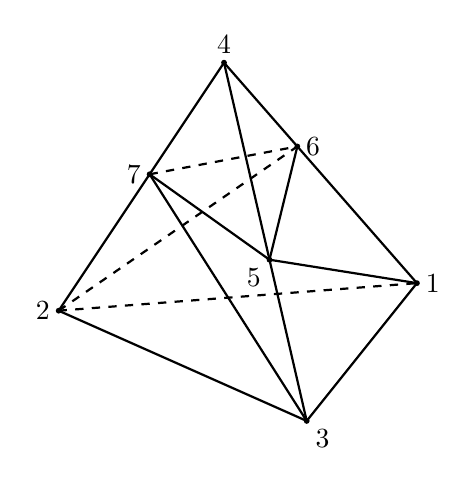
\begin{tikzpicture}[scale=0.7, every node/.style={inner sep=3pt}]
    % 1. 定义外围的四个主顶点
    \coordinate (N4) at (0, 4);
    \coordinate (N2) at (-3, -0.5);
    \coordinate (N3) at (1.5, -2.5);
    \coordinate (N1) at (3.5, 0);

    % 2. 利用比例计算位于边上的点
    \coordinate (N7) at ($(N4)!0.45!(N2)$);
    \coordinate (N6) at ($(N4)!0.38!(N1)$);
    \coordinate (N5) at ($(N4)!0.55!(N3)$);

    % 3. 绘制背面的虚线 (Dashed lines)
    % 删除了 1 和 7 之间的连线
    \draw[dashed, thick] (N2) -- (N1);
    \draw[dashed, thick] (N7) -- (N6);
    \draw[dashed, thick] (N2) -- (N6);

    % 4. 绘制正面的实线边框 (Solid boundary lines)
    \draw[thick] (N4) -- (N7);
    \draw[thick] (N7) -- (N2);
    \draw[thick] (N4) -- (N6);
    \draw[thick] (N6) -- (N1);
    \draw[thick] (N2) -- (N3);
    \draw[thick] (N3) -- (N1);

    % 5. 绘制内部的实线剖分 (Inner solid lines)
    % 删除了 2 和 5 之间的连线，添加了 3 和 7 之间的连线
    \draw[thick] (N4) -- (N5);
    \draw[thick] (N5) -- (N3);
    \draw[thick] (N7) -- (N5);
    \draw[thick] (N6) -- (N5);
    \draw[thick] (N1) -- (N5);
    \draw[thick] (N3) -- (N7); 

    % 6. 绘制顶点圆点及数字标签
    \fill (N4) circle (1.5pt) node[above] {4};
    \fill (N2) circle (1.5pt) node[left] {2};
    \fill (N3) circle (1.5pt) node[below right] {3};
    \fill (N1) circle (1.5pt) node[right] {1};
    \fill (N5) circle (1.5pt) node[below left] {5};
    \fill (N6) circle (1.5pt) node[right] {6};
    \fill (N7) circle (1.5pt) node[left] {7};

\end{tikzpicture}
\end{center}
Show that the toric variety associated to the fan above is complete and nonsingular, and determine whether it is projective or not. 

\begin{solution}
    It is complete and nonsingular but it is not projective. 
    We use notation $\Delta_{ijk}$ to denote the triangulated tetrahedron generated by vertex $v_i,v_j,v_k$ and origin. Let $\Delta_{0123}$ denote the triangulated tetrahedron generated by vertices $v_1,v_2,v_3,v_4$.

    To see the completeness, The decomposition 
    \begin{align*}
        \Delta_{0123} = \Delta_{123}\cup \Delta_{135}\cup \Delta_{156}\cup\Delta_{456}\cup\Delta_{237}\cup\Delta_{357}\cup\Delta_{457}\cup\Delta_{126}\cup\Delta_{267}\cup\Delta_{467}.
    \end{align*}
    implies the completeness. Since it gives a subdivision of $\Delta_{0123}$. Let $Y$ be the toric variety corresponding to the fan generated by $\Delta_{123},\Delta_{134},\Delta_{234},\Delta_{124}$. 
    Clearly, $Y$ is complete and $X(\Delta)$ as the blow-up of $Y$ maintains the completeness.
   
    
    Let determinant of $v_i,v_j,v_k$ denoted by $d_{ijk}$. Then 
    \begin{align*}
        d_{123}=d_{267}=d_{135}=d_{156}=d_{457} = -1 \qquad d_{126}=d_{467}=d_{456}=d_{237}=d_{357}=1
    \end{align*}
    implies the smoothness of $X(\Delta)$.

    Finally, we show that \(X(\Delta)\) is not projective. Suppose, for contradiction, that \(X(\Delta)\) is projective. Then \(\Delta\) admits a strictly convex support function \(\psi\). Put
\[
a_i=\psi(v_i).
\]
Using the linear relations
\[
v_1+v_7=v_2+v_6,
\qquad
v_3+v_6=v_1+v_5,
\qquad
v_2+v_5=v_3+v_7,
\]
and the strict convexity of \(\psi\), we get
\[
a_1+a_7<a_2+a_6,
\qquad 
a_3+a_6<a_1+a_5,
\qquad 
a_2+a_5<a_3+a_7.
\]
Adding these three inequalities gives
\[
(a_1+a_7)+(a_3+a_6)+(a_2+a_5)
<
(a_2+a_6)+(a_1+a_5)+(a_3+a_7),
\]
which is impossible, since the two sides are equal. Hence no strictly convex support function exists on \(\Delta\). Therefore \(X(\Delta)\) is not projective.
\end{solution}


\section*{Problem 4}
For the toric variety $X=\mathbb{P}^{n}$ with its divisors $D_{0},\dots,D_{n}$, verify directly that:
\begin{enumerate}
    \item $D=\sum a_{i}D_{i}$ is generated by its sections $\iff \Psi_{D}$ is convex $\iff a_{0}+\dots+a_{n}\ge0$, and 
    \item $D$ is ample $\iff \Psi_{D}$ is strictly convex $\iff a_{0}+\dots+a_{n}>0$.
\end{enumerate}

\begin{solution}
(1) Let \(X=\mathbb P^n\) with its standard fan. The rays are generated by
\(v_0=-e_1-\cdots-e_n\) and \(v_i=e_i\) for \(1\le i\le n\). The maximal cone
\(\sigma_i\) is generated by all \(v_j\) with \(j\neq i\). Let
\(D=\sum_{i=0}^n a_iD_i\), and put \(s=a_0+\cdots+a_n\).

For the Cartier datum \(m_i=m_{\sigma_i}\), we have
\(\langle m_i,v_j\rangle=-a_j\) for \(j\neq i\). Hence
\(m_0=(-a_1,\dots,-a_n)\), and for \(i\ge1\),
\[
m_i=(-a_1,\dots,-a_{i-1},s-a_i,-a_{i+1},\dots,-a_n).
\]
Thus \(m_i-m_0=s e_i^*\).

Now
\[
P_D=\{m\in M_{\mathbb R}\mid \langle m,v_i\rangle\ge -a_i
\text{ for all }i\}.
\]
The divisor \(D\) is generated by global sections iff \(m_i\in P_D\) for every
maximal cone \(\sigma_i\). For \(m_0\), the only inequality to check is the one
for \(v_0\), and it gives \(s\ge0\). For \(m_i\) with \(i\ge1\), the only
inequality to check is the one for \(v_i\), and it also gives \(s\ge0\).
Therefore
\[
D\text{ is generated by sections}
\Longleftrightarrow \Psi_D\text{ is convex}
\Longleftrightarrow s\ge0.
\]

(2) For strict convexity, the Cartier data on adjacent maximal cones must be
distinct and bend strictly. Since \(m_i-m_0=s e_i^*\), this happens exactly when
\(s>0\). Hence
\[
\Psi_D\text{ is strictly convex}\Longleftrightarrow s>0.
\]
Finally, since \(D_i\sim H\) for all \(i\), we have \(D\sim sH\). Thus
\(\mathcal O(D)\simeq \mathcal O_{\mathbb P^n}(s)\), which is ample iff
\(s>0\). Hence
\[
D\text{ is ample}
\Longleftrightarrow \Psi_D\text{ is strictly convex}
\Longleftrightarrow a_0+\cdots+a_n>0.
\]
\end{solution}

\section*{Problem 5}
Let
\begin{align*}
    A&=\{P\subseteq M_{\mathbb{R}} \mid P \text{ is a full dimensional rational polytope}\},\\
    B&=\{(X(\Delta),D) \mid D \text{ is a } T_{N}\text{-invariant ample divisor in } X(\Delta)\},
\end{align*}
where $\Delta$ is a complete fan, i.e. $|\Delta|=N_{\mathbb{R}}$. Show that the maps $P\mapsto(X_{P},D_{P})$ and $(X(\Delta),D)\mapsto P_{D}$ define bijections between the sets $A$ and $B$ which are inverses of each other.
\begin{solution}
    Let \(P\subset M_{\mathbb R}\) be a full-dimensional rational polytope,
and let \(\Delta_P\) be its normal fan.  Since \(P\) is full-dimensional,
\(\Delta_P\) is complete.  For every ray \(\rho\in\Delta_P(1)\), let
\(v_\rho\in N\) be its primitive generator, and set
\(a_\rho=-\min_{m\in P}\langle m,v_\rho\rangle\).  Define
\(D_P=\sum_{\rho\in\Delta_P(1)}a_\rho D_\rho\).  Then
\[
P=
\{m\in M_{\mathbb R}\mid
\langle m,v_\rho\rangle\ge -a_\rho
\text{ for all }\rho\in\Delta_P(1)\}.
\]
Indeed, these are precisely the facet inequalities of \(P\), so
\(P_{D_P}=P\).  Moreover, the support function
\(\Psi_P(v)=\min_{m\in P}\langle m,v\rangle\) is strictly convex with
respect to the normal fan \(\Delta_P\).  Hence \(D_P\) is ample on
\(X(\Delta_P)\), and the assignment \(P\mapsto (X_P,D_P)\) is
well-defined.

Conversely, let \((X(\Delta),D)\in B\), where
\(D=\sum_{\rho\in\Delta(1)}a_\rho D_\rho\) is an invariant ample divisor.
Define
\[
P_D=
\{m\in M_{\mathbb R}\mid
\langle m,v_\rho\rangle\ge -a_\rho
\text{ for all }\rho\in\Delta(1)\}.
\]
Since \(D\) is ample, its support function \(\Psi_D\) is strictly convex
with respect to \(\Delta\).  Therefore \(P_D\) is a full-dimensional
rational polytope, and its normal fan is exactly \(\Delta\).

It remains to check that the two constructions are inverse.  Starting
from \(P\), the definition of \(D_P\) gives \(P_{D_P}=P\).  Starting from
\((X(\Delta),D)\), the ampleness of \(D\) implies that the normal fan of
\(P_D\) is \(\Delta\).  Moreover, for every ray \(\rho\in\Delta(1)\),
one has \(\min_{m\in P_D}\langle m,v_\rho\rangle=-a_\rho\), since the
inequality \(\langle m,v_\rho\rangle\ge -a_\rho\) defines the
corresponding facet of \(P_D\).  Hence
\[
D_{P_D}
=
\sum_{\rho\in\Delta(1)}a_\rho D_\rho
=
D.
\]
Thus the assignments \(P\mapsto (X_P,D_P)\) and
\((X(\Delta),D)\mapsto P_D\) are inverse bijections.
\end{solution}
\end{document}